\documentclass{article}
%--PASTE INTO MAIN FILE--
% \documentclass{article}
% %--PASTE INTO MAIN FILE--
% \documentclass{article}
% %--PASTE INTO MAIN FILE--
% \documentclass{article}
% \input{TexBase/DocumentBase.tex}
% \end{document}

\usepackage[margin = 0.7in]{geometry}
\usepackage{graphicx}
\usepackage{graphics}
\usepackage[T1]{fontenc}
\usepackage[polish]{babel}
\usepackage{cmap}
\usepackage[utf8]{inputenc}
\usepackage{float}
\usepackage{tabularx}
\usepackage[table,xcdraw]{xcolor}
\usepackage{lipsum}
\usepackage{titlesec}
\usepackage{minted}
\usepackage{xcolor}
\usepackage{caption}
\usepackage{enumitem}
\usepackage{csvsimple}
\usepackage{natbib}
\usepackage{blindtext}

\usepackage{numprint} % rounding
\usepackage[round-precision=3,round-mode=figures, scientific-notation=true]{siunitx} %scientific notation

\usepackage[hidelinks]{hyperref}
\usepackage{url}

\usepackage{bm} %bold for math


%TABS
\usepackage[]{booktabs}
\usepackage{tabularray}
\usepackage{multirow}

%\title{}
\author{Michał Dziedziak, Michał Zychowicz}
\date{\today}


\titlespacing\section{0pt}{12pt plus 4pt minus 2pt}{0pt plus 2pt minus 2pt}
\titlespacing\subsection{0pt}{12pt plus 4pt minus 2pt}{0pt plus 2pt minus 2pt}
\titlespacing\subsubsection{0pt}{12pt plus 4pt minus 2pt}{0pt plus 2pt minus 2pt}
\setlength{\parskip}{\baselineskip}%
\setlength{\parindent}{0pt}%

\newcommand{\squeezeup}{\vspace{-5mm}}


\begin{document}

\begin{titlepage}
    \begin{center}
        \vspace*{5cm}
        \rule{500pt}{1pt}\\
        \vspace*{0.5cm}
        \LARGE
        \textbf{Dokumentacja Projektu}\\
        \Large
        Kamera samochodowa z funkcją wykrywania obiektów i panelem konfiguracyjnym
        \vspace*{0.5cm}
        \rule{500pt}{1pt}
    \end{center}

    \vspace*{10cm}

    {\raggedright
        \large
        \textbf{Autorzy:} Michał Dziedziak 263901, Michał Zychowicz 263950\\
        \textbf{Imię i Nazwisko prowadzącego kurs: mgr inż. Tomasz Serafin} \\
        \textbf{Dzień i godzina zajęć: Wtorek NP, 7:30 - 11:00} 
    }
\end{titlepage}


\tableofcontents
\listoftables

%\renewcommand\listoflistingscaption{List of source codes}
\listoflistings

\listoffigures


\newpage


% \begin{table}[H]
%     \centering
%     \begin{tabular}{|c|c|c|c|}%
%         \hline
%         \bfseries Numer iteracji & \bfseries Czas zalezienia rozwiązania [ms] & Koszt ścieżki & Błąd względny% specify table head
%         \csvreader[head to column names]{Csv/BestPathTest_SimulatedAnnealing_LINEAR_ftv47.csv}{}% use head of csv as column names
%         {\\\hline\Iteration & \num{\TimeInMiliSeconds} & \Cost & \num[round-precision=2, round-mode=places, scientific-notation=false]{\Error}\%}% specify your columns here
%         \\\hline    
%     \end{tabular}
%     \caption{}
%     \label{tab:}
% \end{table}

% \begin{figure}[H]
%     \centering
%     \resizebox{\columnwidth}{!}{%
%     \includegraphics{}%
%     }
%     \caption{}
%     \label{fig:}
% \end{figure}

% \begin{listing}[H]
%     \begin{minted}[frame=single,framesep=2mm,linenos,fontsize=\footnotesize]{language}
%         some code
%     \end{minted}
%     \caption{}
%     \label{lst:}
% \end{listing}


% \bibliographystyle{plainnat}
% \bibliography{TexBase/Bibliography.bib}

% \end{document}

\usepackage[margin = 0.7in]{geometry}
\usepackage{graphicx}
\usepackage{graphics}
\usepackage[T1]{fontenc}
\usepackage[polish]{babel}
\usepackage{cmap}
\usepackage[utf8]{inputenc}
\usepackage{float}
\usepackage{tabularx}
\usepackage[table,xcdraw]{xcolor}
\usepackage{lipsum}
\usepackage{titlesec}
\usepackage{minted}
\usepackage{xcolor}
\usepackage{caption}
\usepackage{enumitem}
\usepackage{csvsimple}
\usepackage{natbib}
\usepackage{blindtext}

\usepackage{numprint} % rounding
\usepackage[round-precision=3,round-mode=figures, scientific-notation=true]{siunitx} %scientific notation

\usepackage[hidelinks]{hyperref}
\usepackage{url}

\usepackage{bm} %bold for math


%TABS
\usepackage[]{booktabs}
\usepackage{tabularray}
\usepackage{multirow}

%\title{}
\author{Michał Dziedziak, Michał Zychowicz}
\date{\today}


\titlespacing\section{0pt}{12pt plus 4pt minus 2pt}{0pt plus 2pt minus 2pt}
\titlespacing\subsection{0pt}{12pt plus 4pt minus 2pt}{0pt plus 2pt minus 2pt}
\titlespacing\subsubsection{0pt}{12pt plus 4pt minus 2pt}{0pt plus 2pt minus 2pt}
\setlength{\parskip}{\baselineskip}%
\setlength{\parindent}{0pt}%

\newcommand{\squeezeup}{\vspace{-5mm}}


\begin{document}

\begin{titlepage}
    \begin{center}
        \vspace*{5cm}
        \rule{500pt}{1pt}\\
        \vspace*{0.5cm}
        \LARGE
        \textbf{Dokumentacja Projektu}\\
        \Large
        Kamera samochodowa z funkcją wykrywania obiektów i panelem konfiguracyjnym
        \vspace*{0.5cm}
        \rule{500pt}{1pt}
    \end{center}

    \vspace*{10cm}

    {\raggedright
        \large
        \textbf{Autorzy:} Michał Dziedziak 263901, Michał Zychowicz 263950\\
        \textbf{Imię i Nazwisko prowadzącego kurs: mgr inż. Tomasz Serafin} \\
        \textbf{Dzień i godzina zajęć: Wtorek NP, 7:30 - 11:00} 
    }
\end{titlepage}


\tableofcontents
\listoftables

%\renewcommand\listoflistingscaption{List of source codes}
\listoflistings

\listoffigures


\newpage


% \begin{table}[H]
%     \centering
%     \begin{tabular}{|c|c|c|c|}%
%         \hline
%         \bfseries Numer iteracji & \bfseries Czas zalezienia rozwiązania [ms] & Koszt ścieżki & Błąd względny% specify table head
%         \csvreader[head to column names]{Csv/BestPathTest_SimulatedAnnealing_LINEAR_ftv47.csv}{}% use head of csv as column names
%         {\\\hline\Iteration & \num{\TimeInMiliSeconds} & \Cost & \num[round-precision=2, round-mode=places, scientific-notation=false]{\Error}\%}% specify your columns here
%         \\\hline    
%     \end{tabular}
%     \caption{}
%     \label{tab:}
% \end{table}

% \begin{figure}[H]
%     \centering
%     \resizebox{\columnwidth}{!}{%
%     \includegraphics{}%
%     }
%     \caption{}
%     \label{fig:}
% \end{figure}

% \begin{listing}[H]
%     \begin{minted}[frame=single,framesep=2mm,linenos,fontsize=\footnotesize]{language}
%         some code
%     \end{minted}
%     \caption{}
%     \label{lst:}
% \end{listing}


% \bibliographystyle{plainnat}
% \bibliography{TexBase/Bibliography.bib}

% \end{document}

\usepackage[margin = 0.7in]{geometry}
\usepackage{graphicx}
\usepackage{graphics}
\usepackage[T1]{fontenc}
\usepackage[polish]{babel}
\usepackage{cmap}
\usepackage[utf8]{inputenc}
\usepackage{float}
\usepackage{tabularx}
\usepackage[table,xcdraw]{xcolor}
\usepackage{lipsum}
\usepackage{titlesec}
\usepackage{minted}
\usepackage{xcolor}
\usepackage{caption}
\usepackage{enumitem}
\usepackage{csvsimple}
\usepackage{natbib}
\usepackage{blindtext}

\usepackage{numprint} % rounding
\usepackage[round-precision=3,round-mode=figures, scientific-notation=true]{siunitx} %scientific notation

\usepackage[hidelinks]{hyperref}
\usepackage{url}

\usepackage{bm} %bold for math


%TABS
\usepackage[]{booktabs}
\usepackage{tabularray}
\usepackage{multirow}

%\title{}
\author{Michał Dziedziak, Michał Zychowicz}
\date{\today}


\titlespacing\section{0pt}{12pt plus 4pt minus 2pt}{0pt plus 2pt minus 2pt}
\titlespacing\subsection{0pt}{12pt plus 4pt minus 2pt}{0pt plus 2pt minus 2pt}
\titlespacing\subsubsection{0pt}{12pt plus 4pt minus 2pt}{0pt plus 2pt minus 2pt}
\setlength{\parskip}{\baselineskip}%
\setlength{\parindent}{0pt}%

\newcommand{\squeezeup}{\vspace{-5mm}}


\begin{document}

\begin{titlepage}
    \begin{center}
        \vspace*{5cm}
        \rule{500pt}{1pt}\\
        \vspace*{0.5cm}
        \LARGE
        \textbf{Dokumentacja Projektu}\\
        \Large
        Kamera samochodowa z funkcją wykrywania obiektów i panelem konfiguracyjnym
        \vspace*{0.5cm}
        \rule{500pt}{1pt}
    \end{center}

    \vspace*{10cm}

    {\raggedright
        \large
        \textbf{Autorzy:} Michał Dziedziak 263901, Michał Zychowicz 263950\\
        \textbf{Imię i Nazwisko prowadzącego kurs: mgr inż. Tomasz Serafin} \\
        \textbf{Dzień i godzina zajęć: Wtorek NP, 7:30 - 11:00} 
    }
\end{titlepage}


\tableofcontents
\listoftables

%\renewcommand\listoflistingscaption{List of source codes}
\listoflistings

\listoffigures


\newpage


% \begin{table}[H]
%     \centering
%     \begin{tabular}{|c|c|c|c|}%
%         \hline
%         \bfseries Numer iteracji & \bfseries Czas zalezienia rozwiązania [ms] & Koszt ścieżki & Błąd względny% specify table head
%         \csvreader[head to column names]{Csv/BestPathTest_SimulatedAnnealing_LINEAR_ftv47.csv}{}% use head of csv as column names
%         {\\\hline\Iteration & \num{\TimeInMiliSeconds} & \Cost & \num[round-precision=2, round-mode=places, scientific-notation=false]{\Error}\%}% specify your columns here
%         \\\hline    
%     \end{tabular}
%     \caption{}
%     \label{tab:}
% \end{table}

% \begin{figure}[H]
%     \centering
%     \resizebox{\columnwidth}{!}{%
%     \includegraphics{}%
%     }
%     \caption{}
%     \label{fig:}
% \end{figure}

% \begin{listing}[H]
%     \begin{minted}[frame=single,framesep=2mm,linenos,fontsize=\footnotesize]{language}
%         some code
%     \end{minted}
%     \caption{}
%     \label{lst:}
% \end{listing}


% \bibliographystyle{plainnat}
% \bibliography{TexBase/Bibliography.bib}



    \section{Opis tematu projektu i planowanego do wykonania systemu}
    \input{Sections/OpisProjektuISystemu.tex}
        
    \section{Case studies}
    \subsection{Sytuacje obsługiwane przez system}

Tworzony system będzie w stanie obsługiwać następujące sytuacje:

\begin{itemize}
	\item Rysowanie pomocniczych linii poziomych
	\begin{itemize}
		\item Na obrazie z kamery rysowane są statyczne linie pomocnicze mające na celu wspomaganie kierowcy przy parkowaniu
		
		\begin{center}
			Zdjęcie poniżej przedstawia przykładową wizualizacje linii pomocniczych
		\end{center}
		
		\begin{figure}[H]
			\centering
			\resizebox{\columnwidth}{!}{
				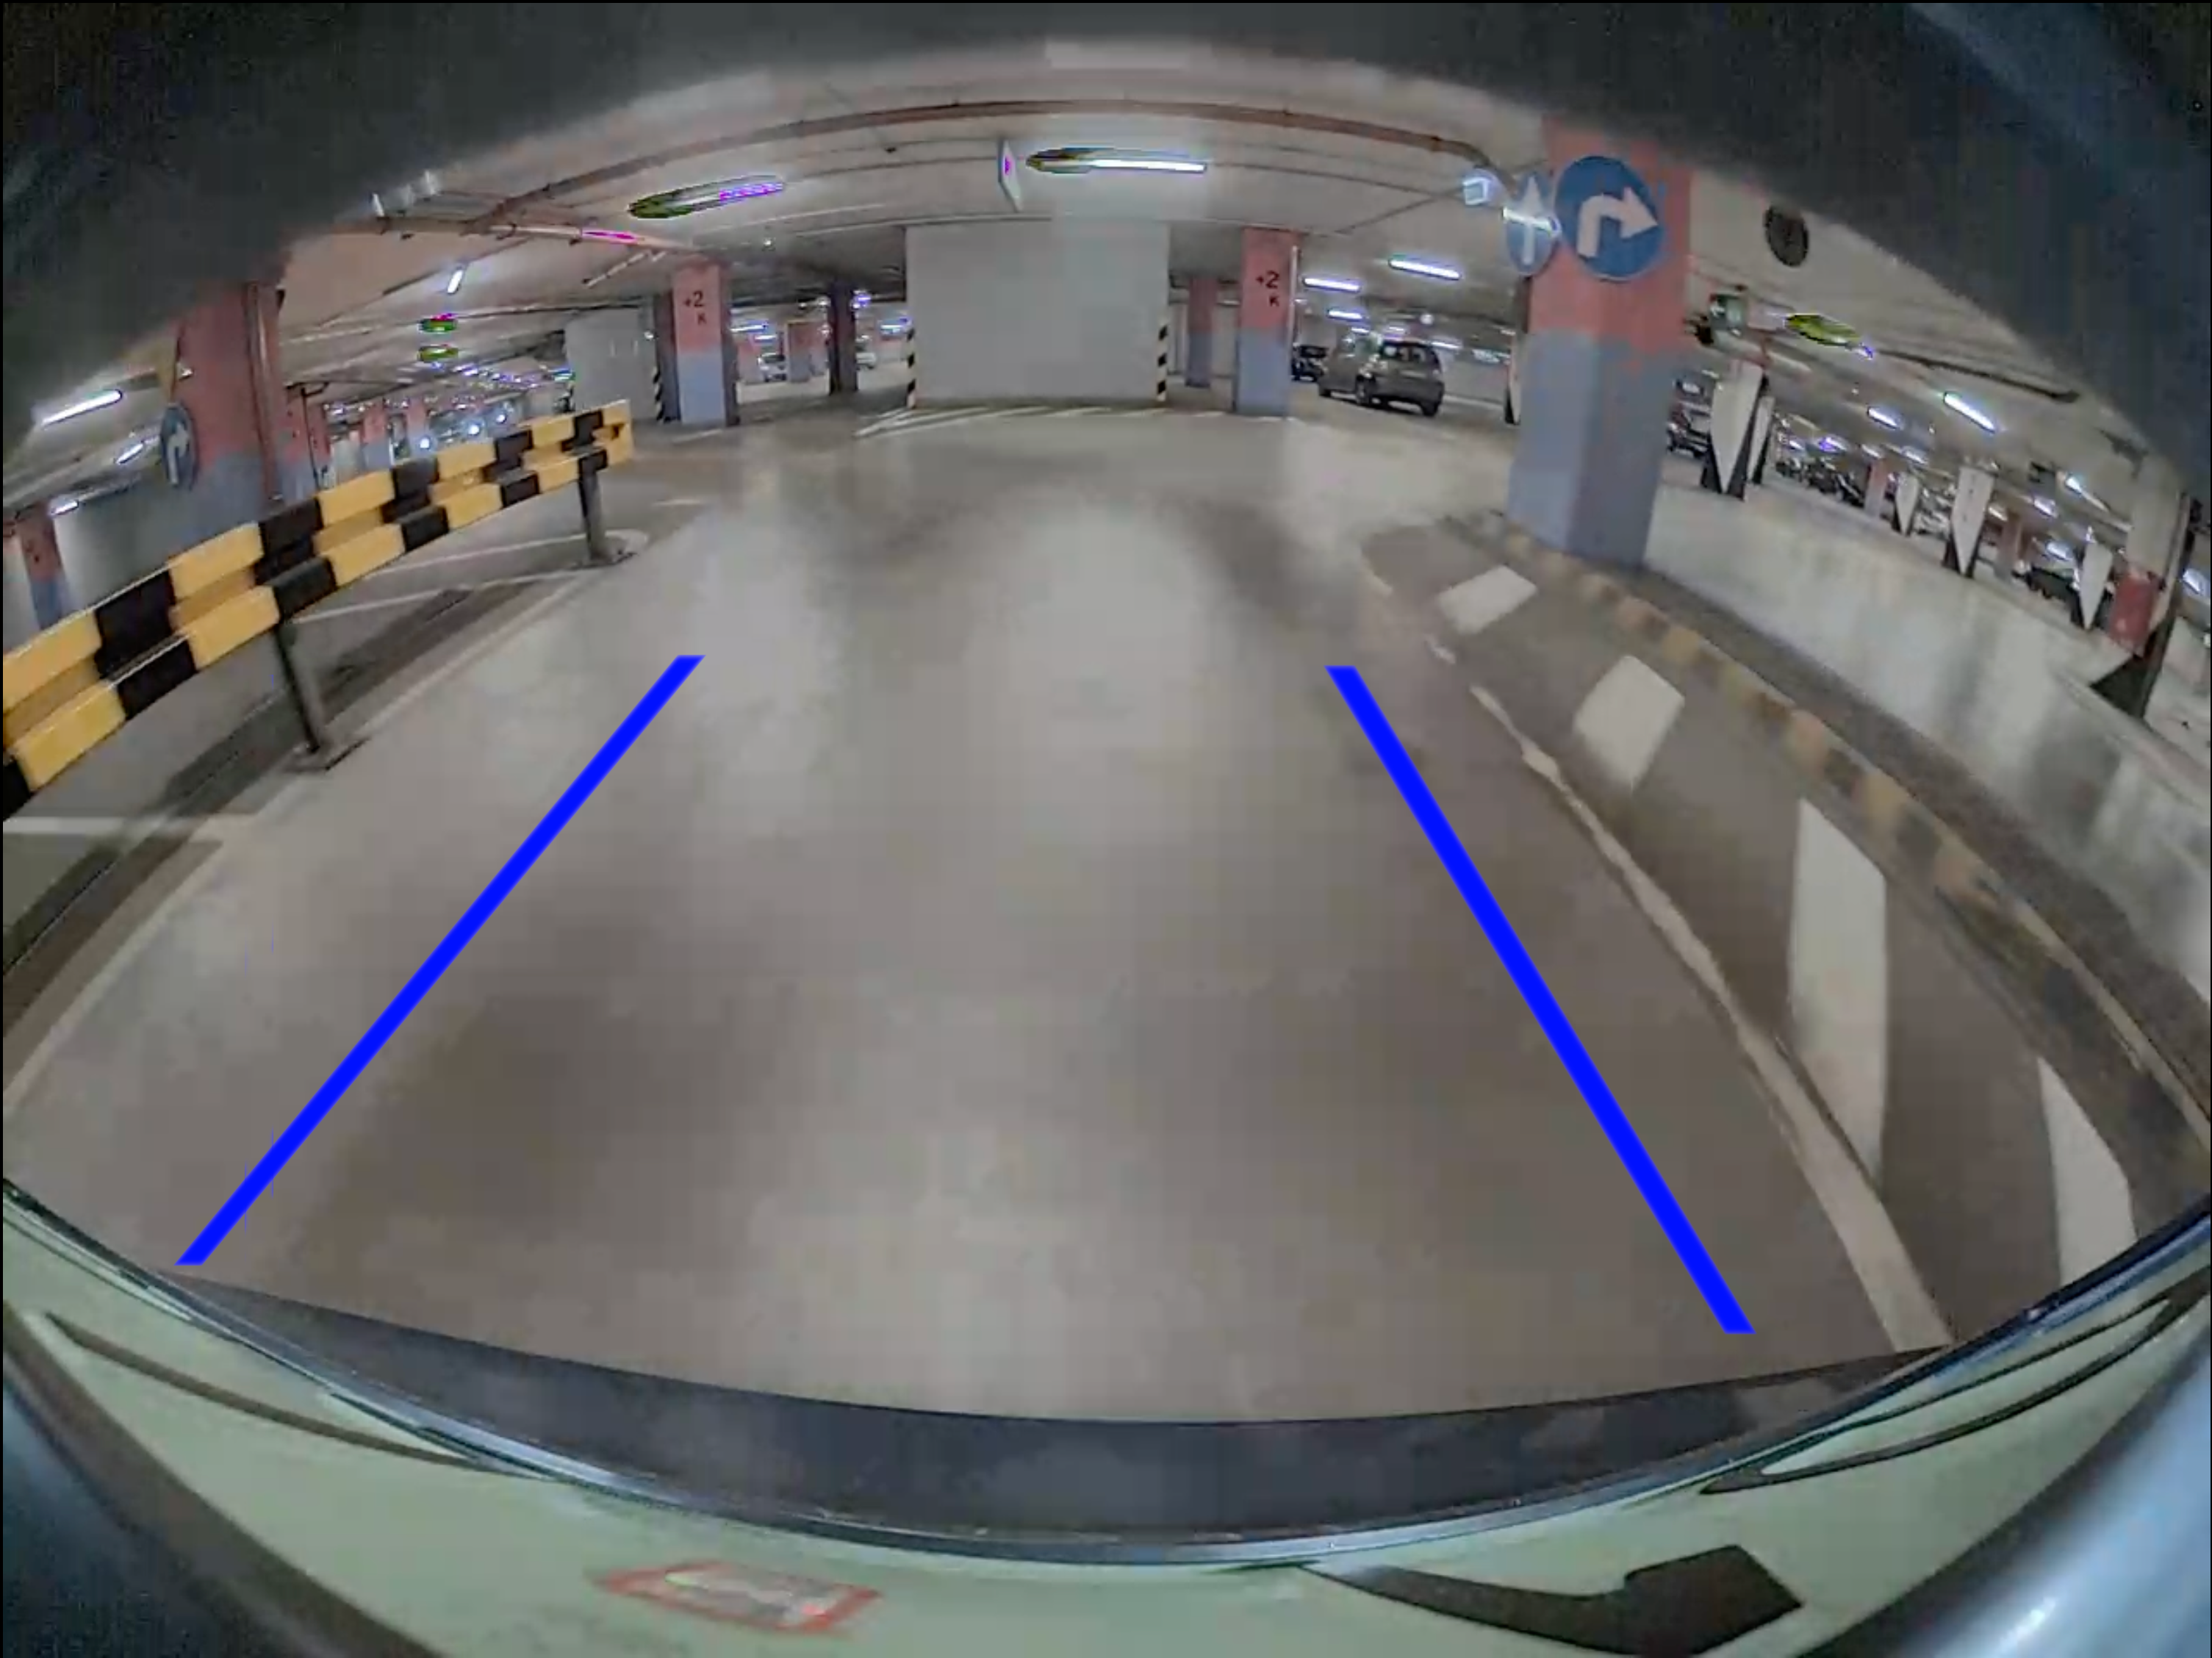
\includegraphics{Img/linie_pomocnicze.png}
			}
			\caption{Linie pomocnicze są nakładane na obraz z kamery}
			\label{fig:linie}
		\end{figure}
	\end{itemize}
	\newpage
	\item Wykrywanie pieszych znajdujących się przed lub za samochodem
	\begin{itemize}
		\item Po wykryciu pieszego w polu widzenia kamery system informuje o tym kierowcę w wybrany w konfiguratorze sposób. \newline
		\begin{center}
			Zdjęcie poniżej pokazuje przykład tego typu sytuacji:
		\end{center}

		\begin{figure}[H]
			\centering
	 		\resizebox{\columnwidth}{!}{
				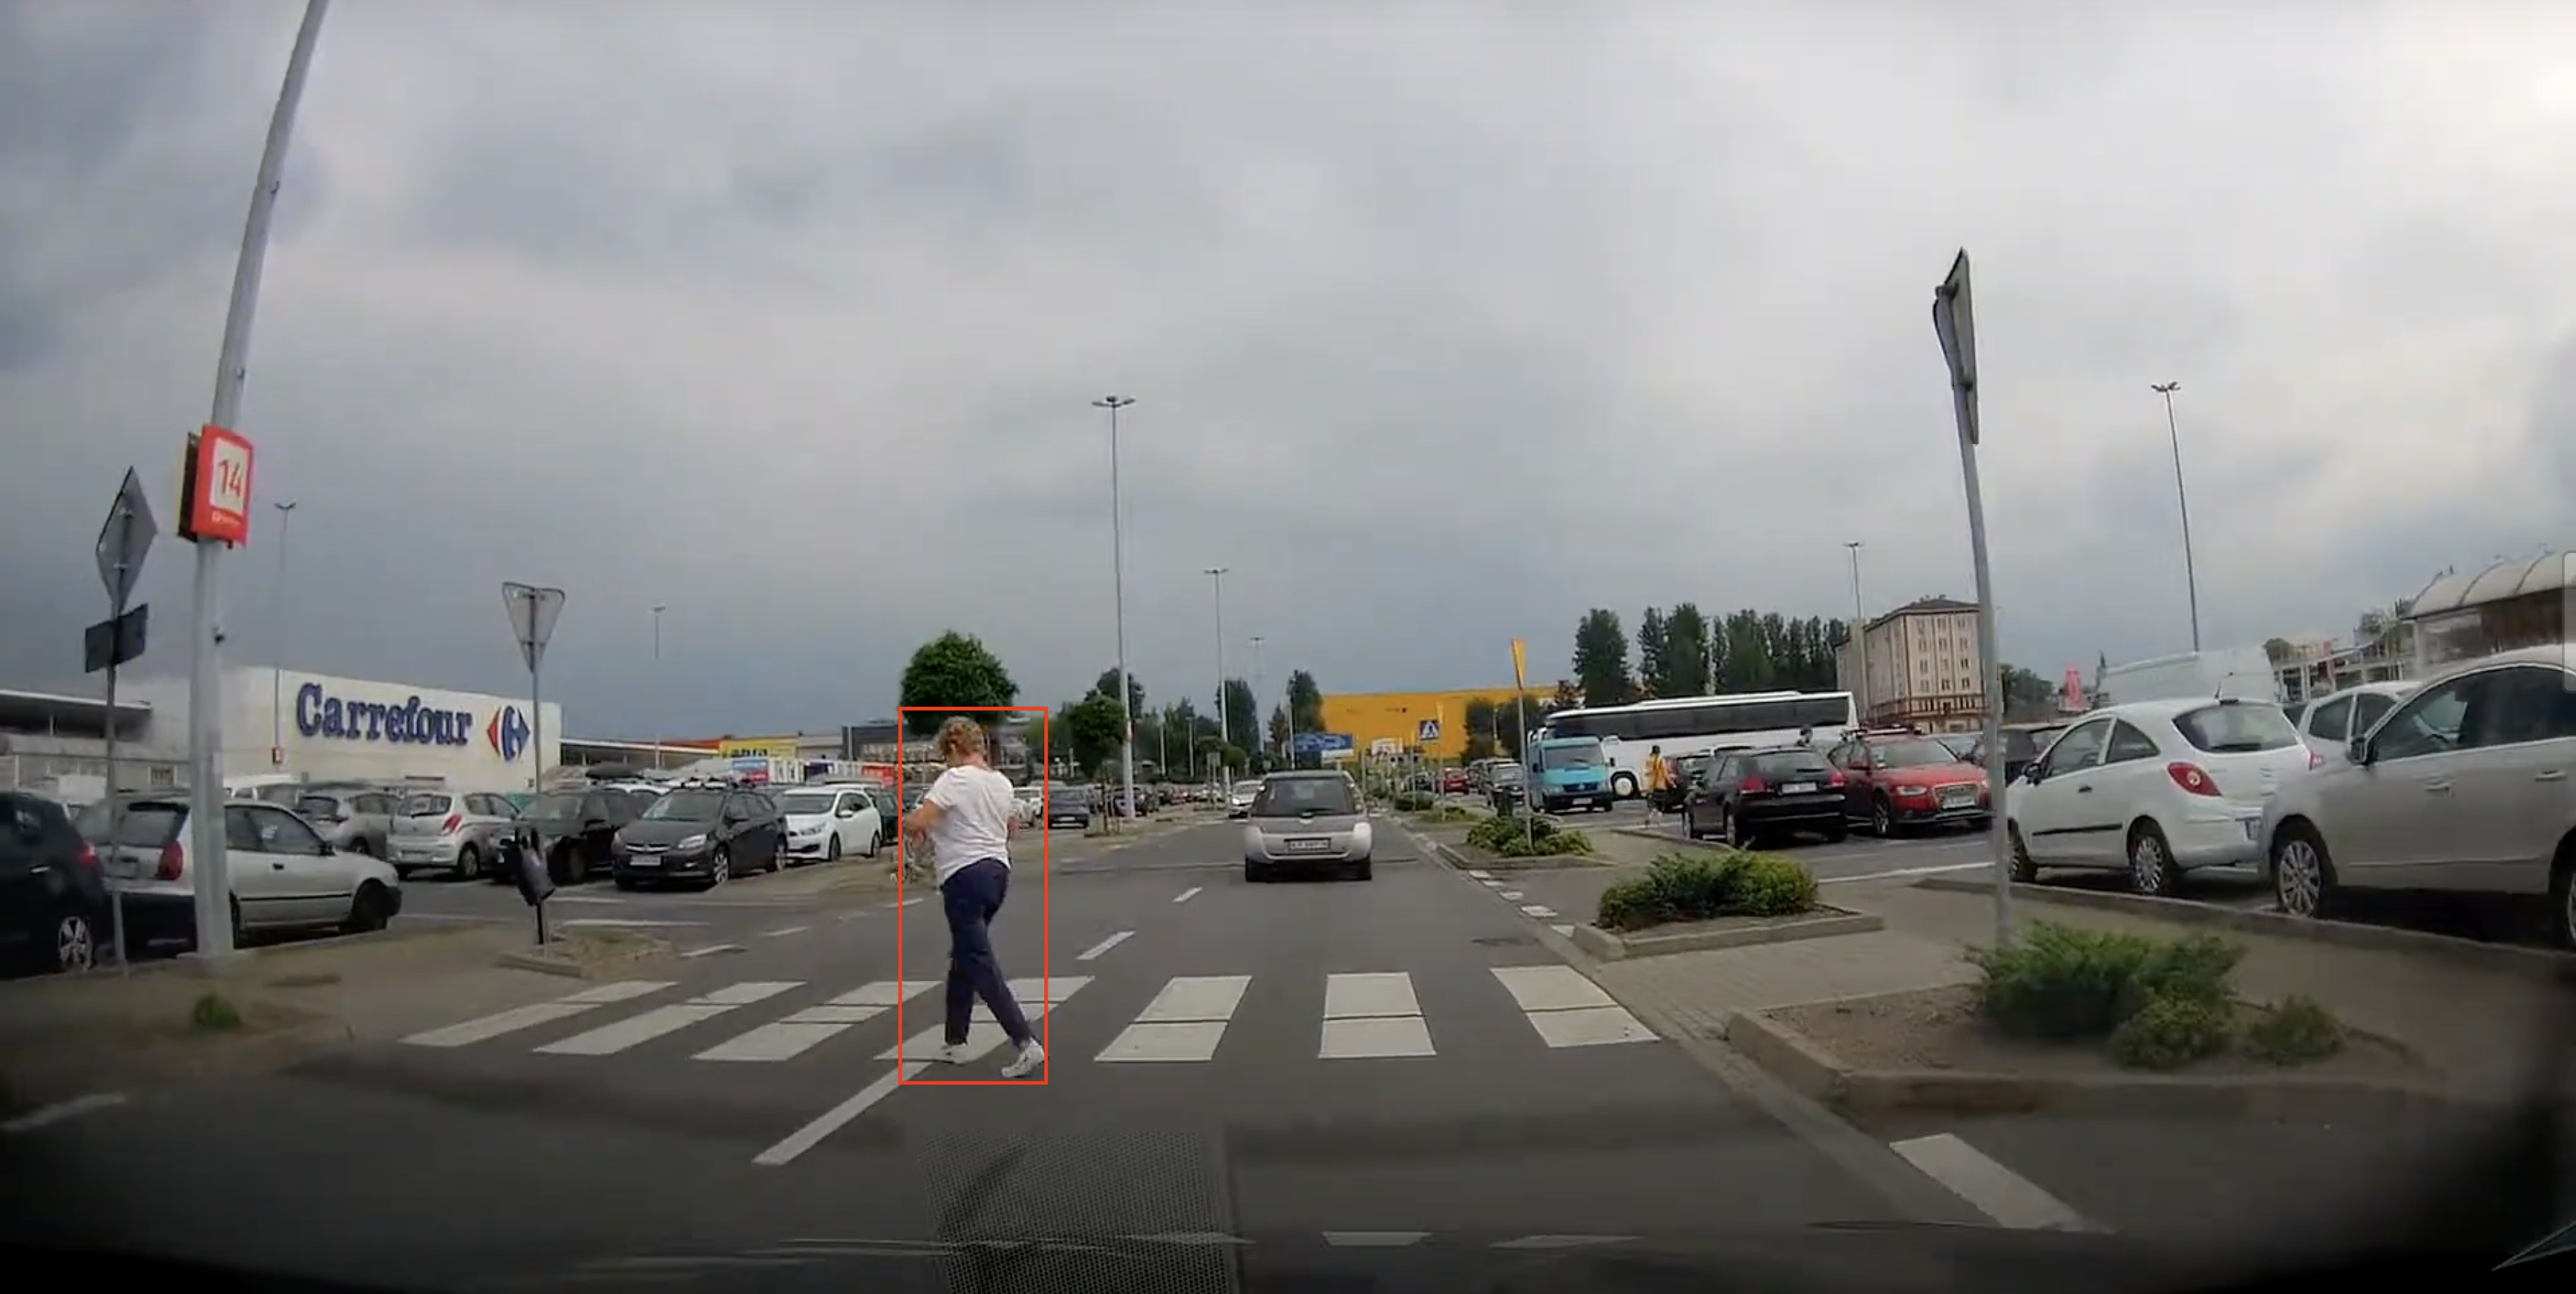
\includegraphics{Img/pieszy.png}
			}
       		\caption{Wykryty pieszy zostaje oznaczony przez system}
			\label{fig:pieszy}
		\end{figure}
	\end{itemize}
	
	\newpage
	
	\item Wykrywanie znaku Stop oraz znaków z grupy znaków ostrzegawczych
	\begin{itemize}
		\item Kiedy w polu widzenia kamery zostanie wykryty jeden z rozpoznawanych znaków kierowca zostanie o tym poinformowany w wybrany w konfiguratorze sposób.
		
		\begin{center}
			Zdjęcie poniżej pokazuje przykład tego typu sytuacji:
		\end{center}
		
		\begin{figure}[H]
			\centering
			\resizebox{\columnwidth}{!}{
				\includegraphics{Img/znak_ostrzegawczy.png}
			}
			\caption{Wykryty znak ostrzegawczy zostaje oznaczony przez system}
			\label{fig:znak}
		\end{figure}
		
	\end{itemize}
	
	\newpage
	
	\item Wykrywanie innych samochodów
	\begin{itemize}
		\item Kiedy system wykryje samochód w polu widzenia kamery, poinformuje on o tym kierowcę, w sposób wybrany w konfiguratorze.
		
		\begin{center}
			Zdjęcie poniżej pokazuje przykład tego typu sytuacji:
		\end{center}
		
		\begin{figure}[H]
			\centering
			\resizebox{\columnwidth}{!}{
				\includegraphics{Img/inny_samochod.png}
			}
			\caption{Wykryty samochód zostaje oznaczony przez system}
			\label{fig:samochod}
		\end{figure}
		
	\end{itemize}
\end{itemize}
  

  


    \section{Opis funkcjonalny}
    System został zaprojektowany w celu skutecznego wykrywania i identyfikacji 
różnych obiektów na drodze, w tym znaków drogowych, pojazdów oraz pieszych. 
Oprócz tego, system oferuje dodatkowe możliwości, które pozwalają na bardziej 
kompleksową obsługę sytuacji drogowych. Poniżej przedstawiamy szczegółowy 
opis funkcjonalny systemu

\begin{itemize}
    \item \textbf{Wykrywanie pojazdów:} System jest zdolny do wykrywania różnych
     typów pojazdów poruszających się na drodze, włączając w to samochody osobowe, 
     ciężarówki oraz inne pojazdy.
    
     \item \textbf{Wykrywanie pieszych:} System jest wyposażony w funkcję wykrywania pieszych 
    poruszających się wzdłuż drogi lub przechodzących przez nią. 
    
    \item \textbf{Wykrywanie ostrzegawczych znaków drogowych:} System umożliwia identyfikację i klasyfikację 
    ostrzegawczych znaków drogowych.

    \item \textbf{Alerty:} System może dawać znać o wykrytych obiektach na różne sposoby, 
    takie jak ramka wokół wykrytego obiektu, czy ostrzeżenie dźwiękowe. 
    
    \item \textbf{Rysowanie lini:} Na ekranie kamery rysowane są linie ułatwiające parkowanie.

    \item \textbf{Konfigurowalne parametry:} Użytkownik ma możliwość konfiguracji parametrów dotyczących 
    wykrywania obiektów, rysowania linii oraz wyświetlania alertów. 
    Może dostosować te parametry do swoich indywidualnych preferencji i potrzeb.

\end{itemize}

    \section{Architektura wysokopoziomowa systemu}
    \subsection{Opis}
System zawiera następujące elementy:
\begin{itemize}
	\item Kamera przednia
	\item Kamera tylna
	\item Komputer
	\item Ekran
	\item Głośnik
\end{itemize}

Obraz z kamer przesyłany jest do komputera, gdzie zostaje on przetworzony, oraz przeprowadzany jest proces wykrywania obiektów. Następnie komputer przesyła przetworzony obraz na ekran, oraz może uruchomić sygnał dźwiękowy jeśli wykryty zostanie określony typ obiektu.



\subsection{Schemat}
    \begin{figure}[H]
	\centering
	\resizebox{\columnwidth}{!}{%
		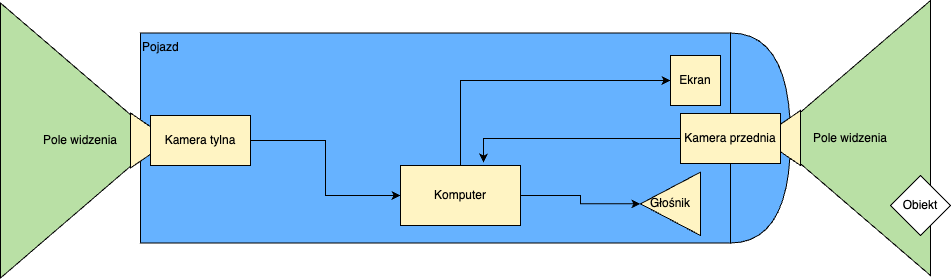
\includegraphics{Img/architektura.png}%
	}
	\caption{Schemat architektury wysokopoziomowej systemu:}
	\label{fig:architektura_diagram}
\end{figure}

    \section{Architektura logiczna systemu}
    \input{Sections/Architektura Logiczna.tex}

    \section{Dobór technologii}
    \input{Sections/DobórTechnologii.tex}

    \section{Planowany zakres prac rozwojowych}
    
\begin{table}[H]
    \centering
    \begin{tabular}{|ccc|l|}
        \hline
        \multicolumn{3}{|c|}{\textbf{Tydzień}}                                                & \multicolumn{1}{c|}{\multirow{2}{*}{\textbf{Zadania}}}                                                                                                          \\ \cline{1-3}
        \multicolumn{1}{|c|}{\textbf{numer}} & \multicolumn{1}{c|}{\textbf{od}} & \textbf{do} & \multicolumn{1}{c|}{}                                                                                                                                           \\ \hline
        \multicolumn{1}{|c|}{1}              & \multicolumn{1}{c|}{2024-03-25}  & 2024-03-31  & \begin{tabular}[c]{@{}l@{}}- Omówienie   tematu \\ - Poszukiwanie pomysłów do realizacji w ramach projektu. \\ - Wybór narzędzi   i technologii\end{tabular}   \\ \hline
        \multicolumn{1}{|c|}{2}              & \multicolumn{1}{c|}{2024-04-01}  & 2024-04-07  & \begin{tabular}[c]{@{}l@{}}- Uszczegółowianie założeń projektowych\\ - Tworzenie dokumentacji.\end{tabular}                                                     \\ \hline
        \multicolumn{1}{|c|}{3}              & \multicolumn{1}{c|}{2024-04-08}  & 2024-04-14  & - Nauka obsługi wybranych narzędzi.                                                                                                                             \\ \hline
        \multicolumn{1}{|c|}{4}              & \multicolumn{1}{c|}{2024-04-15}  & 2024-04-21  & - Produkcja modelu zdolnego do wykrywania obiektów                                                                                     \\ \hline
        \multicolumn{1}{|c|}{5}              & \multicolumn{1}{c|}{2024-04-22}  & 2024-04-28  & - Produkcja modelu zdolnego do wykrywania obiektów                                                                                  \\ \hline
        \multicolumn{1}{|c|}{6}              & \multicolumn{1}{c|}{2024-04-29}  & 2024-05-05  & - Stworzenie szkieletu aplikacji z funkcjonalnością wykrywania obiektów                                                                                         \\ \hline
        \multicolumn{1}{|c|}{7}              & \multicolumn{1}{c|}{2024-05-06}  & 2024-05-12  & - Implementacja funkcjonalności rysowania linii pomocniczych                                                                                                    \\ \hline
        \multicolumn{1}{|c|}{8}              & \multicolumn{1}{c|}{2024-05-13}  & 2024-05-19  & \begin{tabular}[c]{@{}l@{}}- Ogólna weryfikacja spełnienia założeń projektowych.\\ - Kontrola jakości i poprawki związane z użytkowaniem aplikacji\end{tabular} \\ \hline
        \multicolumn{1}{|c|}{9}              & \multicolumn{1}{c|}{2024-05-20}  & 2024-05-26  & - Napisanie i przeprowadzenie testów aplikacji                                                                                                                  \\ \hline
        \multicolumn{1}{|c|}{10}             & \multicolumn{1}{c|}{2024-05-27}  & 2024-06-02  & - Naprawianie błędów                                                                                                                                            \\ \hline
        \multicolumn{1}{|c|}{11}             & \multicolumn{1}{c|}{2024-06-03}  & 2024-06-09  & - Wdrażanie poprawek                                                                                                                                            \\ \hline
    \end{tabular}
    \caption{Tabela przedstawiająca harmonogram pracy na przestrzeni kolejnych tygodni}
    \label{tab:HARMONOGRAM}
\end{table}

    \subsubsection*{Tydzień 1.}
    Pierwszy tydzień zostanie poświęcony na poszukiwanie pomysłów do realizacji w ramach projektu. 
    Po wybraniu kandydatów rozważymy narzędzia i technologie, które zostaną użyte w projekcie.

    \subsubsection*{Tydzień 2.}
    W drugim tygodniu uszczegółowimy założenia projektowe.
    \begin{itemize}
        \item Wybierzemy jakie dokładnie obiekty będą identyfikowane przez nasz system.
        \item Ustalimy w jak będzie informować kierowce o wykrytych obiektach.
        \item Rozważymy strukture aplikacji.
        \item Ustalimy koncept wyglądu aplikacji.
    \end{itemize}
    Następnie przystąpimy do tworzenia dokumentacji.

    \subsubsection*{Tydzień 3.}
    Trzeci tydzień poświęcimy na naukę obsługi wybranych narzędzi.

    \subsubsection*{Tydzień 4., 5.}
    W czwartym i piątym tygodniu skupimy się na produkcji modelu zdolnego do wykrywania 
    interesujących nas obiektów. Pod koniec tego etapu będziemy mieli prostą aplikację
    wyświetlającą nagranie wideo z alertami o wykrytych obiektach.

    \subsubsection*{Tydzień 6.}
    Szósty tydzień poświęcimy na stworzenie szkieletu aplikacji.
    Będzie ona bliska wyglądem docelowej wersji i będzie miała zaimplementowany
    model wykrywający obiekty.

    \subsubsection*{Tydzień 7.}
    W siódmym tygodniu dodamy do aplikacji możliwość rysowanie linii pomocniczych.

    \subsubsection*{Tydzień 8.}
    Podczas ósmego tygodnia zajmiemy się intuicyjnością i wygodą użytkowania aplikacji.
    Dokonamy szlifów interfejsu użytkownika.
    
    \subsubsection*{Tydzień 9.}
    W dziewiątym tygodniu przeprowadzimy testy aplikacji.
    
    \subsubsection*{Tydzień 10.}
    Dziesiąty tydzień poświęcimy na naprawianie błędów wykrytych podczas poprzedniego tygodnia.

    \subsubsection*{Tydzień 11.}
    Ostatni tydzień poświęcimy na wdrażanie poprawek zleconych przez klienta.

    \section{Plan testów systemu}
    \input{Sections/PlanTestówSystemu.tex}


    
\end{document}
